\chapter{ChordReduce}
\label{chapter:chordreduce}


Distributed computing is a current trend and will continue to be the approach for intensive  applications.
We see this in the development of cloud computing \cite{p2p-cloud}, volunteer computing frameworks like BOINC \cite{anderson2004boinc} and Folding@Home \cite{larson2002folding}, and MapReduce  \cite{mapreduce}.
Google's MapReduce  in particular has rapidly become an integral part in the world of data processing.
A user can use MapReduce to take a large problem, split it into small, equivalent tasks and send those tasks to other processors for computation.
The results are sent back to the user and combined into one answer.

Popular platforms for MapReduce, such as Hadoop \cite{hadoop}  \cite{shvachko2010hadoop}, are explicitly designed to be used in large datacenters \cite{hadoopAssumptions} and the majority of research has been focused there.
However, as we have previously mentioned, there are notable issues with a centralized design.

First and foremost is the issue of fault-tolerance.
Centralized designs have a single point of failure \cite{shvachko2010hadoop}.
So long as all computing resources are located in one geographical area or rely on a particular node, a power outage or catastrophic event could interrupt computations or otherwise disrupt the platform \cite{babaoglu2014people}.

A centralized design assumes that the network is relatively unchanging and may not have mechanisms to handle node failure during execution or, conversely, cannot speed up the execution of a job by adding additional workers on the fly.
Many environments also anticipate a certain degree in homogeneity in the system.
Finally deploying these systems and developing programs for them has an extremely steep learning curve.

There is no reason that these assumptions need to be the case for MapReduce, or for many distributed computing frameworks in general.
Moving away from the data center context opens up more possibilities for distributed computing, such as P2P clouds \cite{p2p-cloud}.
However, without a centralized framework, the network needs some kind of protocol to organize the various components in the network.
As part of our research, we developed a highly robust and distributed MapReduce framework based on Chord, called ChordReduce \cite{chordreduce}.

It is a system that can scale, is fault tolerant, has a minimal amount of latency, and distributes tasks evenly.  
ChordReduce leverages the underlying protocol from Chord \cite{chord} to distribute Map and Reduce tasks to nodes evenly, provide greater data redundancy, and guarantee a greater amount of fault tolerance. 
Rather than viewing Chord solely as a means for sharing files, we see it as a means for distributing work. We established the effectiveness of using Chord as a framework for distributed programming. At the same time we avoid the architectural and file system constraints of systems like Hadoop.  


\section{Background}
ChordReduce takes its name from the two components it is built upon.
Chord \cite{chord} provides the backbone for the network and the file system, providing scalable routing, distributed storage, and fault-tolerance.   
MapReduce runs on top of the Chord network and utilizes the underlying features of the distributed hash table.  This section provides an extensive and expanded background on Chord and MapReduce.


\subsection{Chord}
\label{sec:chord-detail}
We introduced Chord in Chapter \ref{chapter:background}, but we present it here again in greater depth.
Chord \cite{chord} is a P2P protocol for file sharing that uses a hash function to assign addresses to nodes and files for a ring overlay. 
The Chord protocol takes in some key and returns the identity (ID) of the node responsible for that key.  

As we have mentioned discussed in Chapter \ref{chapter:background}, these keys can be generated by hashing a value of the node, such as the IP address and port, or by hashing the filename of a file.  
The hashing process creates a $m$-bit hash identifier.

The nodes are then arranged in a ring from the lowest hash-value to highest.  Chord takes the files and places each in the node that has the same hashed identifier as it.  If no such node exists, the node with the first identifier that follows this value is selected. Since the overlay is a circle, this assignment is computed in modulo $2^m$ space.  

The node responsible for the key $\kappa$ is called the $successor$ of $\kappa$, or $successor(\kappa)$.  For example, if there were some portion of the network with nodes 20, 25, and 27, node 25 would be responsible for the files with the keys (21,22,23,24,25). If node 25 were to decide to leave the network, its absence would be detected by node 27, who would then be responsible for all the keys node 25 was covering, in addition to its own keys. 
\begin{figure}
	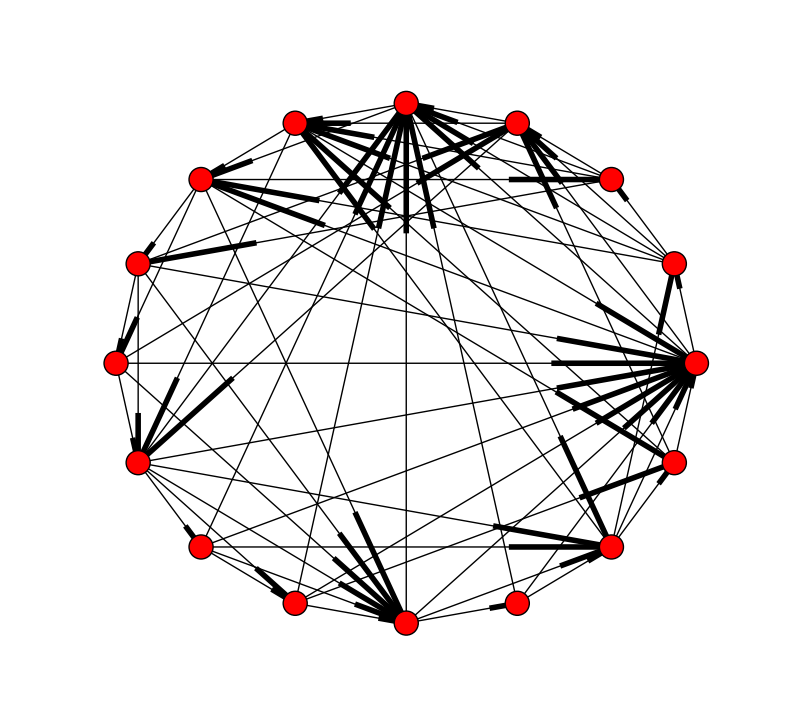
\includegraphics[width=\linewidth]{figs/chordreal}
	\caption{A Chord ring with 16 nodes.  The bold lines are incoming edges.  Each node has a connection to its successor, as well as 4 fingers, some of which are duplicates.}
	\label{fig:chordreal}
\end{figure}


With this scheme, we can reliably find the node responsible for some key by asking the next node in the circle for the information, who would then pass the request through the circle until the successor was found.  We can then proceed to directly connect with the successor to retrieve the file.  This naive approach is largely inefficient, and is a simplification of the lookup process, but it is the basis of how Chord theoretically works.

To speed up the lookup time, each node builds and maintains a \emph{finger table}.  The \emph{finger table} contains the locations of up to $m$ other nodes in the ring.  The $i$th entry of node $n$'s \emph{finger table} corresponds to the node that is the $successor(n+2^{i-1})$ $mod$ $2^m$. Hash values are not perfectly distributed, it is possible to have duplicate entries in the \emph{finger table}. An example Chord network with fingers is shown in in Fig. \ref{fig:chordreal}.


\begin{figure}
	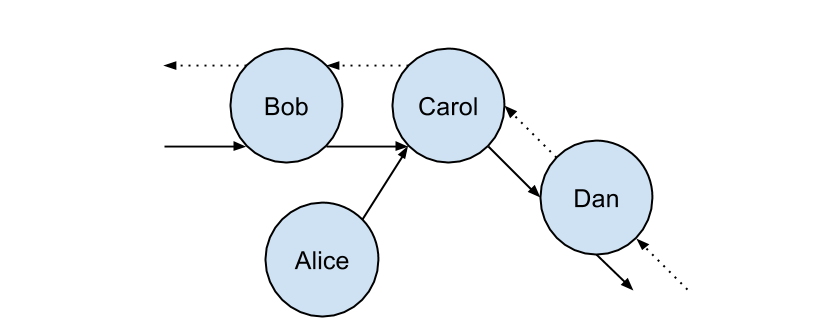
\includegraphics[width=\linewidth]{figs/abcd1}
	\caption{Alice has incorrectly determined that Carol is her appropriate successor.  When Alice stabilizes, Carol will let her know about Bob.}
	\label{fig:abcd1}
\end{figure}


\begin{figure}
	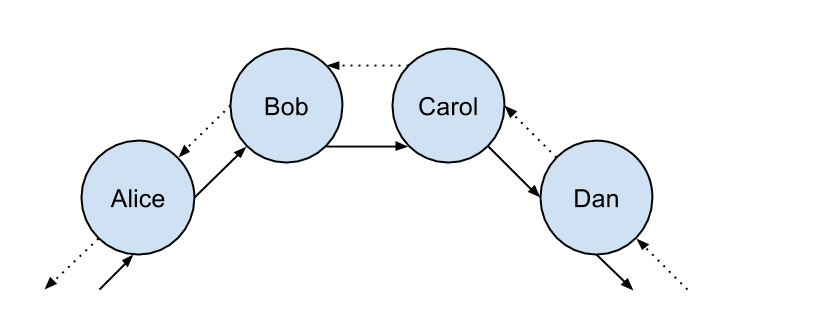
\includegraphics[width=\linewidth]{figs/abcd2}
	\caption{After completing stabilize, Alice makes Bob her successor and notifies him. Bob then made Alice as his predecessor.}
	\label{fig:abcd2}
\end{figure}



When a node $n$ is told to find some key, $n$ looks to see if the key is between $n$ and $successor(n)$ and return $successor(n)$'s information to the requester. 
If not, it looks for the entry in the finger table for the closest preceding node $n'$ it knows and asks $n'$ to find the successor.
This allows each step to skip up to half the nodes in the network, giving a $\log_2(n)$ lookup time.
Because nodes can constantly join and leave the network, each entry in the table is periodically checked and updated during a finger maintenance period. 

To join the network, node $n$ first asks $n'$ to find $successor(n)$ for it.  
Node $n$ uses the information to set his successor, but the other nodes in the ring will not acknowledge $n$'s presence yet.  
Node $n$ relies on the stabilize routine to fully integrate into the ring.

The stabilize routine helps the network integrate new nodes and route around nodes who have left the network. 
Each node periodically checks to see who their successor's predecessor is.  In the case of a static network, this would be the checking node.  
However, if the checking node gets back a different node, it looks at that returned node's ID and changes its own successor if needed.  

Regardless of whether the checking node changes its successor, that node then notifies the (possibly) new successor,  who then checks if he needs to change his predecessor based on this new information.  
While complex, the stabilization process is no more expensive than a heartbeat function.  A more concrete example:

Suppose Alice, Bob, Carol, and Dan are members of the ring and everyone is ordered alphabetically (Fig. \ref{fig:abcd1}). 
Alice is quite sure that Carol is her successor.  
Alice asks Carol who her predecessor is and Carol says Bob is.  
Since Bob is closer to Alice than Carol, Alice changes her successor to Bob and notifies him.  

When Bob sees that notification, he can see Alice is closer than whoever his previous predecessor is and sets Alice to be his predecessor.  
During the next stabilization cycle, Alice will see that she is still Bob's predecessor and notify him that she's still there (Fig. \ref{fig:abcd2}).

To prevent loss of data due to churn, each node sends a backup of their data to their successor, or multiple successors upstream.  
Section \ref{sec:chordreduce-robust} discusses the implementation of the backup process in ChordReduce and expands upon it for backing up Map and Reduce tasks.


\subsection{Extensions of Chord}

The Cooperative File System (CFS) is an anonymous, distributed file sharing system built on top of Chord \cite{CFS}.  
In CFS, rather than storing an entire file at a single node, the file is split up into multiple chunks around 10 kilobytes in size.
These chunks are each assigned a hash and stored in nodes corresponding to their hash in the same way that whole files are.  
The node that would normally store the whole file instead stores a \emph{key block}, which holds the hash address of the chunks of the file. 

The chunking allows for numerous advantages.  
First, it promotes load balancing. 
Each piece of the overall file would (ideally) be stored in a different node, each with a different backup or backups.  
This would prevent any single node from becoming overwhelmed from fulfilling multiple requests for a large file.  
It would also prevent retrieval from being bottlenecked by a node with a relatively low bandwidth. 
Finally, when Chord uses some sort of caching scheme like that described in CFS \cite{CFS}, caching chunks as opposed to the entire file resulted in about 1000 times less storage overhead.  

Mutable files and IRM, which is short for Integrated File Replication and Consistency Maintenance \cite{irm}, has nodes keep track of file requests they initiate or forward.  
If nodes find they are frequently forwarding a request for a particular file, they store that file locally until it is no longer requested frequently.  

Chunking also opens up the options for implementing additional redundancy such as erasure codes \cite{rizzo1997effective}. 
With erasure codes, redundant chunks are created but any combination of a particular number of chunks is sufficient to recreate the file.  
For example, a file that would normally be split into 10 chunks might be split into 15 encoded chunks.  The retrieval of any 10 of those 15 chunks is enough to recreate the file.  
Implementing erasure codes would presumably make a DHT more fault tolerant, but that is an exercise left for future work.


Generally, related files should be kept together for quick retrieval; Chord, however, just hashes the filename to find the responsible node and sends it to that location without any thought to organization.  
One solution to this is to use allow the file owner to select the first $ \beta $ bits of a file's hash, then generating the remaining least significant bits by hashing the filename.  
It does not matter if a file owner, in some infinitesimally small coincidence, chooses the same $ \beta $ bit prefix as another file owner, as the purpose is to keep related files together.   


\subsection{MapReduce}
At its core, MapReduce \cite{mapreduce} is a system for division of labor, providing a layer of separation between the programmer and the more complicated parts of concurrent processing.
The programmer sends a large task to a master node, who then divides that task among slave nodes (which may further divide the task).  This task has two distinct parts: Map and Reduce.  
Map performs some operation on a set of data and then produces a result for each Map operation.  
The resulting data can then be reduced, combining these sets of results into a single set, which is further combined with other sets.
This process continues until one set of data remains.
A core concept here is the tasks are distributed to the nodes that already contain the relevant data, rather than the data and task being distributed together among arbitrary nodes.

The archetypal example of using MapReduce is WordCount -- the task of counting the occurrence of each word in a collection of documents.
These documents have been split up into blocks and stored on the network over the distributed file system.  
The master node locates the worker nodes with blocks and sends the Map and Reduce tasks associated with WordCount.  
Each worker then goes through their blocks and creates a small word frequency list.  
These lists are then used by other workers, who combine them into larger and larger lists, until the master node is left with a word frequency list of all the words in the documents. 

The most popular platform for MapReduce is Hadoop \cite{hadoop}. 
Hadoop is an open-source Java implementation developed by Apache and Yahoo! \cite{pavlo2009comparison}.  
Hadoop has two components, the Hadoop Distributed File System (HDFS) \cite{hdfs} and the Hadoop MapReduce Framework \cite{mrsurvey}.  
Under HDFS, nodes are arranged in a hierarchical tree, with a master node, called the NameNode, at the top.  
The NameNode's job is to organize and distribute information to the slave nodes, called DataNodes.  
This makes the NameNode a single point of failure \cite{shvachko2010hadoop} in the network, as well as a potential bottleneck for the system \cite{hadoop-bottle}.

To do work on Hadoop, the user stores their data on the network.  
This is handled by the NameNode, which equally apportions the data among the DataNodes.  
When a user wants to run some analysis on the data or some subset the data, then that function is sent by the NameNode to each of the DataNodes that is responsible for the indicated data.   
After the DataNode finishes processing, the result is handled by other nodes called Reducers which collect and reduce the results of multiple DataNodes.



\section{Related Work}

We have identified two papers that focus on combining P2P concepts with MapReduce.  Both papers are similar to our research, but differ in crucial ways, as described below.

%DEFINE ISSUES OF CHURN AND RELIABLILITY

\subsection{P2P-MapReduce}
Marozzo et al. \cite{marozzo2012p2p} investigated the issue of fault tolerance in centralized MapReduce architectures such as Hadoop.  They focused on creating a new P2P based MapReduce architecture built on JXTA \cite{jxta} called P2P-MapReduce.  P2P-MapReduce is designed to be more robust at handling node and job failures during execution.

Rather than use a single master node, P2P-MapReduce employs multiple master nodes, each responsible for some job.  If one of those master nodes fails, another will be ready as a backup to take its place and manage the slave nodes assigned to that job.  This avoids the single point of failure that Hadoop is vulnerable to. Failures of the slave nodes are handled by the master node responsible for it.

Experimental results were gathered via simulation and compared P2P-MapReduce to a centralized framework. Their results showed that while P2P-MapReduce generated an order of magnitude more messages than a centralized approach, the difference rapidly began to shrink at higher rates of churn.  When looking at actual amounts of data being passed around the network, the bandwidth required by the centralized approach greatly increased as a function of churn, while the distributed approach again remained relatively static in terms of increased bandwidth usage.  

They concluded that P2P-MapReduce would, in general, use more network resources than a centralized approach. However, this was an acceptable cost as the P2P-MapReduce would lose less time from node and job failures \cite{marozzo2012p2p}.

While P2P-MapReduce is decentralized, it still relies on a very definite master/slave hierarchy for organization, computations, and scaling. 
During simulation, 1\% of the entire network was assigned as master nodes. This means for a simulation of 40000 nodes, 400 were required to organize and coordinate jobs, rendering them unable to do any processing.  In addition, a loosely-consistent Distributed Hash Table (DHT) such as JXTA can be much slower and fails to maintain the same level of guarantees as an actual DHT, such as Chord \cite{5359174}.   


%The loosely-consistent DHT can be much slower than using an acutal DHT such as Chord .
%Scalability.  A huge issue would be tracking all the nodes and coordinating them. Scalability is handled by mainataining a ratio of masters to slaves 
%Evaluated for low rates of churn.  Such low rates also mean master nodes are barely affected by churn.
%Simulations 
%Our work differs from Marozzo et al.'s in that P2P-MapReduce does not examine using the underlying strengths of a particular P2P protocol or group of protocols, which would have made the architecture simpler.  P2P-MapReduce is decentralized, but still relies on a very definite master/slave hierarchy, while all nodes in ChordReduce are both workers and masters.  We also implemented our MapReduce system rather than simulating the work.

\subsection{MapReduce using Symphony}

Lee et al.'s work \cite{leemap} draws attention to the fact that a P2P network can be much more than a way to distribute files and demonstrates how to accomplish different tasks using Map and Reduce functions over a P2P network.  Rather than using Chord, Lee et al. used Symphony \cite{symphony}, another DHT protocol with a ring topology.  To run a MapReduce job over the Symphony ring, a node is selected by the user to effectively act as the master.  This ad-hoc master then performs a bounded broadcast over a subsection the ring.  Each node repeats this broadcast over a subsection of that subsection, resulting in a tree with the first node at the top.  Map tasks are disseminated evenly throughout the tree and their results are reduced on the way back up to the ad-hoc master node.  This allows the ring to disseminate Map and Reduce tasks without the need for a coordinator responsible for distributing these tasks and keeping track of them, unlike Hadoop.

Their experimental results showed that the latency experienced by a centralized configuration is similar to the latency experienced in a completely distributed framework.  However, there are no mechanisms in place to handle churn in the network.  If a node joins during a MapReduce job, it will be unable to contribute any of its resources to the problem. If a node in the bounded broadcast tree fails, or worse the ad-hoc master node fails, the data that node is responsible for is lost. 


\section{ChordReduce}
Marozzo et al. \cite{marozzo2012p2p} shows that adding additional fault-tolerance features to a MapReduce architecture is worth the added cost of maintenance, as the time lost due to node failures is greatly reduced.  However, Marozzo et al. do not explore the benefits of leveraging the properties of a P2P protocol to reduce the complexity of the architecture and completely distribute the responsibility of the task across the network.  As a result, P2P-MapReduce still relies on a ratio of masters to slaves to coordinate and organize the network, meaning a percentage of the network is unable to contribute processing power to the actual solving of a problem.   

Lee et al. \cite{leemap} explores the benefits of building a MapReduce module to run on top of Symphony \cite{symphony},  a P2P protocol.  Unlike Hadoop, this allows the MapReduce tasks to be executed without the need of a central source of coordination by distributing tasks over a bounded broadcast tree created at runtime.  The Symphony based MapReduce architecture would be greatly improved by the addition of components to handle the failure of nodes during execution.  As it stands now, if a node crashes the job will fail due to the loss of data.

While both of these papers have promising results and confirm the capability of our own framework, both solely look at P2P networks for the purpose of routing data and organizing the network. Neither examines using a P2P network as a means of efficiently distributing responsibility throughout the network and using existing features to add robustness to nodes working on Map and Reduce tasks.  

ChordReduce uses Chord to act as a completely distributed topology for MapReduce, negating the need to assign any explicit roles to nodes or have a scheduler or coordinator.  ChordReduce does not need to assign specific nodes the task of backing up work; nodes backup their tasks using the same process that would be used for any other data being sent around the ring.  Finally, results work their way back to a specified hash address, rather than a specific hash node, eliminating any single point of failure in the network.  These features help prevent a bottleneck from occurring. The result is a simple, distributed, and highly robust architecture for MapReduce.


\subsection{Handling Node Failures in Chord}
\label{sec:chordreduce-robust}
Due to the potentially volatile nature of a peer-to-peer network, Chord has to be able to handle (or at the very least, tolerate) an arbitrary amount of churn.  Section \ref{sec:chord-detail} described how Chord gradually guides nodes into their correct locations after they join the network.  The same is true for when a node leaves the network; the stabilize procedure will guide nodes to their correct successors and predecessors.  However, we can exert more control over how to handle nodes leaving the network.

When a node $n$ changes his successor, $n$ asks if the successor is holding any data $n$ should be responsible for.  The successor looks at all the data $n$ is responsible for and sends it to $n$.  The successor does not have to delete this data. In fact, keeping this data as a backup is beneficial to the network as a whole, as $n$ could decide to leave the network at any point. 

Chord specifies two ways a node can leave the ring.  A node can either suddenly drop out of existence, or a node can tell the network he is about to leave, letting his successor and predecessor immediately perform the needed changes.

When a node politely quits, he informs both his successor and predecessor and gives them all the information they need to fill the resulting gap. He also sends all of the data he is responsible for to his successor, who becomes responsible for that data when the node leaves.  Fingers that pointed to that node would be corrected during the finger maintenance period.  This allows for the network to adjust to churn with a minimum of overhead.

It is unlikely that every time a node leaves the network, it will do so politely.  If a node suddenly quits, the data it had stored is lost. To prevent data from becoming irretrievable, a node periodically sends backups to its successor.  In order to prevent a cascade of backups of backups, the node only passes along what it considers itself responsible for.  What a node is responsible for changes as nodes enter and leave the network.  If a node's successor leaves, the node sends a backup to his new successor. 

Our prototype framework does not implement a polite disconnect;  when a node quits, it does so quickly and abruptly.  This design ensures that the  system would be able to handle churn under the worst of cases.  Polite quit could be implemented quite easily.


\subsection{Implementation}

\begin{figure}
	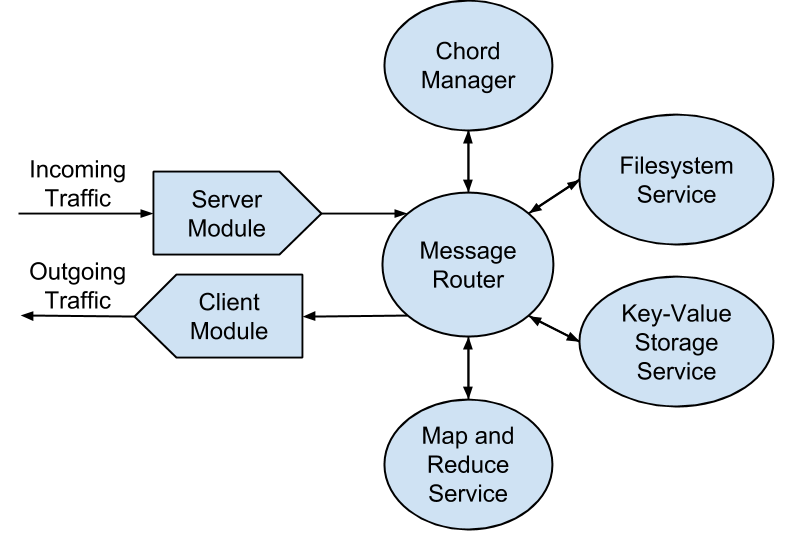
\includegraphics[width=\linewidth]{figs/crArch}
	\caption{The basic architecture of a node in ChordReduce.  MapReduce runs as a service on top of each node.}
	\label{fig:crArch}
\end{figure}

ChordReduce is a fully functional Chord implementation in Python.  Our installation was designed to be as simple as possible.  It consists of downloading our code \cite{chordreduce-code} and running \texttt{chord.py}.  A user can specify a port and IP of a node in the ring they wish to join.  The node will automatically integrate into the ring with this minimal information.  The ring as implemented is stable and well organized.  We created various services to run on top the network, such as a file system and distributed web server.  Our file system is capable of storing whole files or splitting the file up among multiple nodes the ring.  Our MapReduce module is a service that runs on top of our Chord implementation, similar to the file system (Fig. \ref{fig:crArch}).  We avoided any complicated additions to the Chord architecture; instead we used the protocol's properties to create the features we desired in our MapReduce framework. 

In our implementation of MapReduce, each node takes on responsibilities of both a worker and master, much in the same way that a node in a P2P file-sharing service will act as both a client and a server.  Jobs still must start from a single location.  To start a job, the user contacts a node at a specified hash address and provides it with the tasks and data.  This address can be chosen arbitrarily or be a known node in the ring. The node at this hash address is designated as the stager.  

The job of this stager is to take the work and divide it into \emph{data atoms}, which are the smallest individual units that work can be done on.  This might be a line of text in a document, the result of a summation for a particular intermediate value, or a subset of items to be sorted.  The specifics of how to divide the work are defined by the user in a \emph{stage} function.  The data atoms are then each given a random hash and sent to the node responsible for that hash address, guaranteeing they are evenly distributed throughout the network.  The data atoms also contain the Map function and Reduce function as defined by the user.  A job ID is also included, so that data atoms from different jobs can be differentiated.  Once the data atoms are sent out, the stager's job is done and it behaves like any other node in the network. The staging period is the only time ChordReduce is vulnerable to churn, and only if the stager leaves the ring in the middle of sending out data atoms.  The user would get some results back, but only for the data the stager managed to send out.

Nodes that receive data atoms apply the Map function to the data to create result data atoms, which are then sent back to the stager's hash address (or some other user defined address).  This will take $\log_{2} n$ hops traveling over Chord's fingers.  At each hop, the node waits a predetermined minimal amount of time to accumulate additional results (In our experiments, this was 100 milliseconds).

Nodes that receive at least two results merge them using the Reduce function.  The results are continually merged until only one remains at the hash address of the stager. 

Once the reductions are finished, the user retrieves his results from the node at the stager's address.  This may not be the stager himself, as the stager may no longer be in the network.  The stager does not need to collect the results himself, since the work is sent to the stager's hash address, rather than the stager itself.  Thus, the stager could quit the network after staging, and both the user and the network would be unaffected by the change. % Here, we are leverging two features. First, we use the automatic assignment of responsibility to automatically route the data to the sucessor.  %Second, the same process Chord uses to backup files is used to backup the intermediate data. 

Similar precautions are taken for nodes working on Map and Reduce tasks.  Those tasks are backed up by a node's successor, who will run the task if the node leaves before finishing its work (e.g. the successor loses his predecessor).   The task is given a timeout by the node.  If the backup node detects that the responsible node has failed, he starts the work and backs up again to \emph{his} successor.  Otherwise, the data is tossed away once the timeout expires. This is done to prevent a job being submitted twice.

An advantage of our system is the ease of development and deployment.  The developer does not need to worry about distributing work evenly, nor does he have to worry about any node in the network going down.  The stager does not need to keep track of the status of the network.  The underlying Chord ring handles that automatically.  If the user finds they need additional processing power during runtime, they can boot up additional nodes, which would automatically be assigned work based on their hash value.   If a node goes down while performing an operation, his successor takes over for him.  This makes the system extremely robust during runtime.

All a developer needs to do is write three functions: the staging function, Map, and Reduce.  These define how to split up the work into manageable portions, the work to be performed on each portion to obtain results, and how to combine these results into a single result, respectively. 



\section{Experiments}
In order for ChordReduce to be a viable framework, we had to show these three properties:
\begin{enumerate}
	\item ChordReduce provides significant speedup during a distributed job.
	\item ChordReduce scales.
	\item ChordReduce handles churn during execution.
\end{enumerate}
Speedup can be demonstrated by showing that a distributed job is generally performed more quickly than the same job handled by a single worker.  More formally we need to establish that $\exists n$ such that $T_{n} < T_{1}$, where $T_{n}$ is the amount of time it takes for $n$ nodes to finish the job.

To establish scalability, we need to show that the cost of distributing the work grows logarithmically with the number of workers.  In addition, we need to demonstrate that the larger the job is, the number of nodes we can have working on the problem without the overhead incurring diminishing returns increases. This can be stated as $$T_{n} = \frac{T_{1}}{n} + k \cdot \log_{2}(n)$$ where $\frac{T_{1}}{n}$ is the amount of time the job would take when distributed in an ideal universe and $k \cdot \log_{2}(n)$ is network induced overhead, $k$ being an unknown constant dependent on network latency and available processing power.

Finally, to demonstrate robustness, we need to show that ChordReduce can handle arbitrary node failure in the ring and that such failures minimally impair the overall speed of the network.

\subsection{Setup}

\begin{figure}
	\centering
	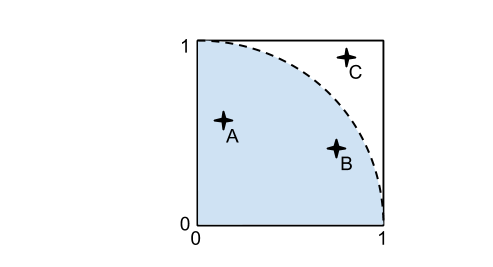
\includegraphics[width=0.5\linewidth]{figs/dartboard}
	\caption{The "dartboard." The computer throws a dart by choosing a random $x$ and $y$ between 0 and 1.  If $x^{2} + y^{2} < 1^{2} $, the dart landed inside the circle.  $A$ and $B$ are darts that landed inside the circle, while $C$ did not.}
	\label{fig:dartboard}
\end{figure}

To stress test our framework, we ran a Monte-Carlo approximation of $\pi$. This process is largely analogous to having a square with the top-right quarter of a circle going through it (Fig. \ref{fig:dartboard}), and then throwing darts at random locations.  Counting the ratio of darts that land inside the circle to the total number of throws gives us an approximation of $\frac{\pi}{4}$.  The more darts thrown, i.e. the more samples that are taken, the more accurate the approximation\footnote{This is not intended to be a particularly good approximation of $\pi$. Each additional digit of accuracy requires increasing the number of samples taken by an order of magnitude.}.

We chose this experiment for a number of reasons. The job is extremely easy to distribute.  This also made it very easy to test scalability. By doubling the amount of samples, we can double the amount of work each node gets.  We could also test the effectiveness of distributing the job among different numbers of workers.

Each Map job is defined by the number of throws the node must make and yields a result containing the total number of throws and the number of throws that landed inside the circular section.  Reducing these results is then a matter of adding the respective fields together. 

We ran our experiments using Amazons's Elastic Compute Cloud (EC2) service.  Amazon EC2 allows users to purchase an arbitrary amount of virtual machines by the hour. Each node was an individual EC2 small instance \cite{amazon-instances} with a preconfigured Ubuntu 12.04 image.  These instances were capable enough to provide constant computation, but still weak enough that they would be overwhelmed by traffic on occasions, creating a constant churn effect in the ring.  

Once started, nodes retrieve the latest version of the code and run it as a service, automatically joining the network.  We can choose any arbitrary node as the stager and tell it to run the MapReduce process. We found that the network was robust enough that we could take a node we wanted to be the stager out of the network, modify its MapReduce test code, have it rejoin the network, and then run the new code without any problems. Since only the stager has to know how to create the Map tasks, the other nodes do not have to be updated and execute the new tasks they are given.

We ran our experiments on groups of 1, 10, 20, 30, and 40 workers, which generated a $10^{8}$ sample set and a $10^{9}$ sample set.  Additionally, we gathered data on a $10^{7}$ sample set using 1, 5, 10, 20, 30 workers.  To test churn, we ran an experiment where each node had an equal chance of leaving and joining the network and varied the level of churn over multiple runs.  

We also utilized a subroutine we wrote called $plot$, which sends a message sequentially around the ring to establish how many members there are.  If $plot$ failed to return in under a second, the ring was experiencing structural instability.

\subsection{Results}

\begin{figure}
	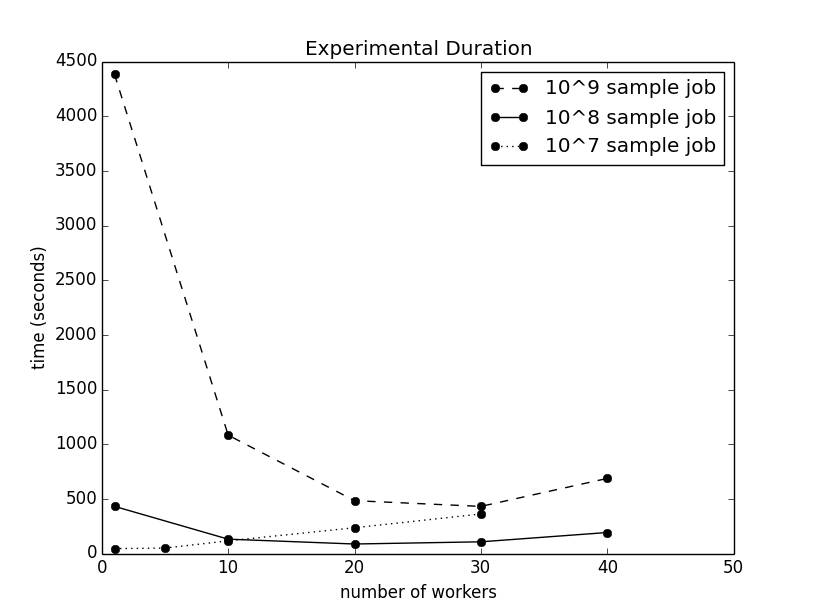
\includegraphics[width=\linewidth]{figs/expTime}
	\caption{For a sufficiently large job, it was almost always preferable to distribute it.  When the job is too small, such as with the $10^{7}$ data set, our runtime is dominated by the overhead.  Our results are what we would expect when overhead grows logarithmically to the number of workers.}
	\label{fig:expTime}
\end{figure}


\begin{figure}
	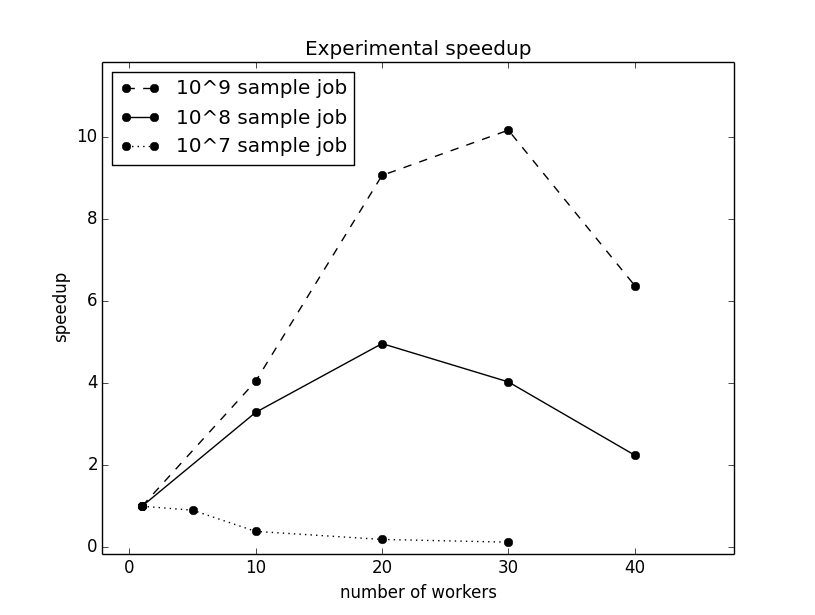
\includegraphics[width=\linewidth]{figs/expSpeed}
	\caption{The larger the size of the job, the greater the gains of distributing with ChordReduce.  In addition, the larger the job, the more workers can be added before we start seeing diminishing returns.  This demonstrates that ChordReduce is scalable.}
	\label{fig:expSpeed}
\end{figure}

Fig. \ref{fig:expTime} and Fig. \ref{fig:expSpeed} summarize the experimental results of job duration and speedup.  Our default series was the $10^{8}$ samples series.  On average, it took a single node 431 seconds, or approximately 7 minutes, to generate $10^{8}$ samples.  Generating the same number of samples using ChordReduce over 10, 20, 30, or 40 nodes was always quicker.  The samples were generated fastest when there were 20 workers, with a speedup factor of 4.96, while increasing the number of workers to 30 yielded a speedup of only 4.03.  At 30 nodes, the gains of distributing the work were present, but the cost of overhead ($k \cdot \log_{2}(n)$) had more of an impact.  This effect is more pronounced at 40 workers, with a speedup of 2.25.

Since our data showed that approximating $\pi$ on one node with $10^{8}$ samples took approximately 7 minutes, collecting $10^{9}$ samples on a single node would take 70 minutes at minimum.  Fig. \ref{fig:expSpeed} shows that the $10^{9}$ set gained greater benefit from being distributed than the $10^{8}$ set, with the speedup factor at 20 workers being 9.07 compared to 4.03.  In addition, the gains of distributing work further increased at 30 workers and only began to decay at 40 workers, compared with the $10^{8}$ data set, which began its drop off at 30 workers. This behavior demonstrates that the larger the job being distributed, the greater the gains of distributing the work using ChordReduce.

The $10^{7}$ sample set confirms that the network overhead is logarithmic.  At that size, it is not effective to run the job concurrently and we start seeing overheard acting as the dominant factor in runtime.  This matches the behavior predicted by our equation, $T_{n} = \frac{T_{1}}{n} + k \cdot \log_{2}(n)$. For a small $T_{1}$, $\frac{T_{1}}{n}$  approaches 0 as $n$ gets larger, while $k \cdot \log_{2}(n)$, our overhead, dominates the sample.  The samples from our data set fit this behavior, establishing that our overhead increases logarithmically with the number of workers.


\begin{figure}
	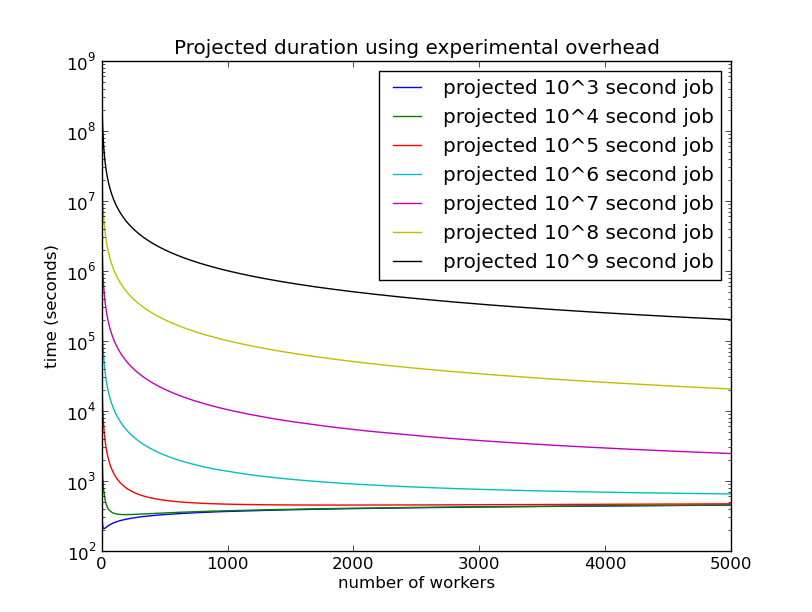
\includegraphics[width=\linewidth]{figs/projTime}
	\caption{The projected runtime using ChordReduce for differently sized jobs.  Each curve projects the expected behavior for job that takes a single worker the specified amount of time.}
	\label{fig:projTime}
\end{figure}

\begin{figure}
	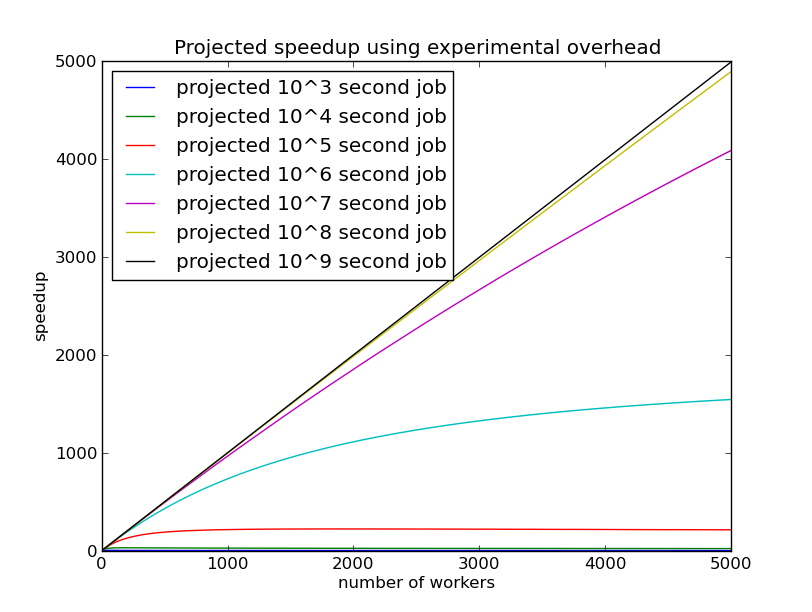
\includegraphics[width=\linewidth]{figs/projSpeed}
	\caption{The projected speedup for different sized jobs. }
	\label{fig:projSpeed}
\end{figure}

Since we have now established that $T_{n} = \frac{T_{1}}{n} + k \cdot \log_{2}(n)$, we can estimate how long a job that takes an arbitrary amount of time to run on a single node would take using ChordReduce.  Our data points indicated that the mean value of $k$ for this problem was 36.5.  Fig. \ref{fig:projTime} shows that for jobs that would take more than $10^{4}$ seconds for single worker to complete, we can expect there would still be benefit to adding an additional worker, even when there are already 5000 workers already in the ring.  Fig. \ref{fig:projSpeed} further emphasizes this. Note that as the jobs become larger, the expected speedup from ChordReduce  approaches linear behavior.


\begin{table}
	\centering
	\begin{tabular}{|r|r|r|} 
		\hline 
		Churn rate per second & Average runtime (s) & Speedup vs 0\% churn\\ \hline{}
		0.8\% & 191.25 & 2.15 \\ \hline
		0.4\% & 329.20 & 1.25 \\ \hline
		0.025\% & 431.86 & 0.95 \\ \hline 
		0.00775\%  & 445.47 & 0.92 \\ \hline 
		0.00250\% & 331.80  &  1.24 \\ \hline 
		0\% & 441.57 & 1.00 \\ \hline
	\end{tabular}
	\caption{} 
	\label{tab:churnSpeed}
\end{table}


Table \ref{tab:churnSpeed} shows the experimental results for different rates of churn. These results show the system  is relatively insensitive to churn.  We started with 40 nodes in the ring and generated $10^{8}$ samples while experiencing different rates of churn, as specified in Table \ref{tab:churnSpeed}.  At the 0.8\% rate of churn, there is a 0.8\% chance each second that any given node will leave the network followed by another node joining the network at a different location. The joining rate and leaving rate being identical is not an unusual assumption to make \cite{marozzo2012p2p} \cite{load}.  

Our testing rates for churn are an order of magnitude higher than the rates used in the P2P-MapReduce simulation  \cite{marozzo2012p2p}.  In their paper, the highest rate of churn was only 0.4\% per minute. Because we were dealing with fewer nodes, we chose larger rates to demonstrate that ChordReduce could effectively handle a high level of churn.  


Our experiments show that for a given problem, ChordReduce can effectively distribute the problem, yielding a substantial speedup.  Furthermore, our results showed that the larger the problem is, the more workers could be added before diminishing returns were incurred.  During runtime, we experienced multiple instances where $plot$ would fail to run and the stager would report socket errors, indicating that it had lost connection with a node in the ring.  Despite this turbulence, every node managed to reestablish connection with each other and report back all the data.  This further demonstrated that we were able to handle the churn in the network.


\section{Remarks}


During our experiments testing the capabilities of ChordReduce, we experienced a significant and completely unexpected anomaly while testing churn.
One of the things previous research \cite{marozzo2012p2p}  \cite{leemap} in the same area we felt we needed to explore better was how a completely decentralized computation could handle churn.
Now, despite our initial prototype having numerous bugs and only able to handle small networks, we were fairly certain of it's ability to handle churn.

Marozzo et al.\ \cite{marozzo2012p2p} tested their network using churn rates of 0.025\%, 0.05\%, 0.1\%, 0.2\%, and 0.4\% per minute.
The churn rate of $cr << 1$ per minute means that each minute on average, $cr \cdot n$ nodes leave the network and $cr \cdot n$  new nodes join the network.\footnote{It is standard practice to assume the joining rate and leaving rate are equal.}
This could effectively be thought of as each node flipping a weighted coin every minute.
When the coin lands on tails, the node leaves.
A similar process happens for nodes wanting to join the network.

We wanted the robustness of our system to be beyond reproach, so we tested at rates from 0.0025\% to 0.8\% \textbf{\textit{per second}}, 120 times the fastest rate used to test P2P-MapReduce.
This is an absurdly fast and unrealistic speed, the only purpose of which was to cement the fault tolerance of the system.
Since we were testing ChordReduce on Amazon's EC2 and paying per instance per hour, we limited the number of nodes.
Rather than having a pool of nodes waiting to join the network, we conserved our funds by having leaving nodes immediately rejoin the network under a new IP/port combo.
The meant our churn operation was essentially a simultaneous leave and join.


What we found was that jobs on ChordReduce finished twice as fast under the unrealistic levels churn (0.8\% per second) than no churn (Table \ref{tab:churnSpeed}).
This completely mystified us.
Churn is a disruptive force; how can it be aiding the network?

\subsection*{Hypothesis}
We hypothesize this was due to the number of data pieces (larger) vs the number of workers (smaller).
There were more workers than there were pieces of data, so some workers ended up with more data than others in the initial distribution.
This means that there was some imbalance in the way data was distributed among nodes.
This was \textit{further} exacerbated by small number of workers distributed over a large hash space, leading some nodes to have larger swaths of responsibility than others.

Given this setup, without any churn, the operation would be:
Workers get triggered, they start working, and the ones with little work finish their work quickly, and the network waits for the node with higher loads of work.

Its important to note here that the work in ChordReduce was performed atomically, a piece at a time.
When a node was working on a piece, it informed it's successor, then informed them when it finished.
These pieces of work were also small, possibly too small.

As mentioned previously, under our induced experimental churn, we had the nodes randomly fail and immediately join under a new IP/port combination, which yields a new hash.
The failure rates were orders of magnitude higher than what would be expected in a ``real'' (nonexperimental) environment.
The following possibilities could occur:
\begin{itemize}
	\item A node without any active jobs leaves.
	It dies and and comes back with a new port chosen.
	This new ID has a higher chance of landing in a larger region of responsibility (since new joining nodes have a greater chance of hashing to a larger region than a smaller).
	In other words, it has a (relatively) higher chance of moving into an space where it becomes acquires responsibility for enqueued jobs.
	The outcomes of this are:
	\begin{itemize}
		\item The node rejoins in a region and does not acquire any new jobs.
		This has no impact on the network (Case I).
		\item The node rejoins in a region that has jobs waiting to be done.
		It acquires some of these jobs.
		This speeds up performance (Case II).
	\end{itemize}
	\item A node with active jobs dies.
	It rejoins in a new space.
	The jobs were small, so not too much time is lost on the active job, and the enqueued jobs are backed up and the successor knows to complete them.
	However, the node can rejoin in a more job-heavy region and acquire new jobs.
	The outcomes of this are:
	\begin{itemize}
		\item A minor negative impact on runtime and load balancing (since the successor has more jobs to handle) (Case III).
		\item A possible counterbalance in load balancing by acquiring new jobs off a busy node (Case IV).
	\end{itemize}
\end{itemize}

The longer the nodes work on the jobs, the more nodes finish and have no jobs.
This means as time increases, so do the occurrences of Case I and II.


This leads us to two hypotheses:
\begin{itemize}
	\item Deleting nodes motivates other nodes to work harder to avoid deletion (a ``beatings will continue until morale improves'' situation).
	\item Our high rate of churn was dynamically load-balancing the network.
	It appears even the smallest effort of trying to dynamically load balance, such as rebooting random nodes to new locations, has benefits for runtime.
	Our method is a poor approximation of dynamic load-balancing, and it still shows improvement.
\end{itemize}

The first hypothesis is mentally pleasing to anyone who has tried to create a distributed system, but lacks rigor.
Verification, analysis, and exploitation of this phenomena is  the subject of (Chapter \ref{chapter:auto-balance}).


Once we have established that it does exist, we need a better load-balancing strategy than randomly inducing.
We want nodes to have a precomputed list of locations in which they can insert nodes to perform load-balancing on an ad-hoc basis during runtime.
This precomputed list ties directly into the security research on DHTs we have done \cite{sybil-analysis} and is the subject of Chapter \ref{chapter:sybil}.